\documentclass{article}
\usepackage{graphicx} % Required for inserting images
\usepackage{booktabs}
\usepackage{float}
\usepackage{url}
\usepackage[numbers]{natbib}
\usepackage{amsmath}
\usepackage{graphicx}

\title{Portfolio 2}
\author{Michael Robinette}
\date{October 2026}

\begin{document}

\maketitle

\section*{Data Construction and Description}
For this project, we are working with data collected by the Vermont Data Collaborative \citep{vtdatacollab}, which is a project dedicated to helping Vermont's rural communities by providing data-related services and insights. The data for this project came directly from their database. In this project we will examine whether or not there is a predictive relationship between a home's flood zone status, it's footprint measured in acres, and its assessed value, which is our outcome.

As we see in Figure \ref{fig:assessed_value_vs_lot_size_montpelier}, acreage appears to affect assessed value. However, the impact of flood zone status on a home's assessed value is unclear. We will implement a multiple regression Stan model to explore this further.

\begin{table}[h]
\centering
\begin{tabular}{l l p{0.55\textwidth}}
\toprule
Field & Type & Description \\
\midrule
\texttt{listed\_real\_value} & integer (\$) & Total assessed value from the town grand list (outcome). \\
\texttt{improvements\_value} & integer (\$) & Assessed value of buildings on the parcel; used to drop parcels with no assessed home. \\
\texttt{acres} & float & Parcel size in acres. (predictor) \\
\texttt{n\_homes} & integer & Number of residential building footprints inside the parcel. We filter the dataset such that n\_homes is 1. \\
\texttt{in\_sfha} & binary (0/1) & 1 if any of those footprints intersects a FEMA Special Flood Hazard Area. (predictor) \\
\bottomrule
\end{tabular}
\caption{Data fields and types queried from Vermont Data Collaborative}
\label{tab:fields}
\end{table}

\begin{figure}[H]
\centering
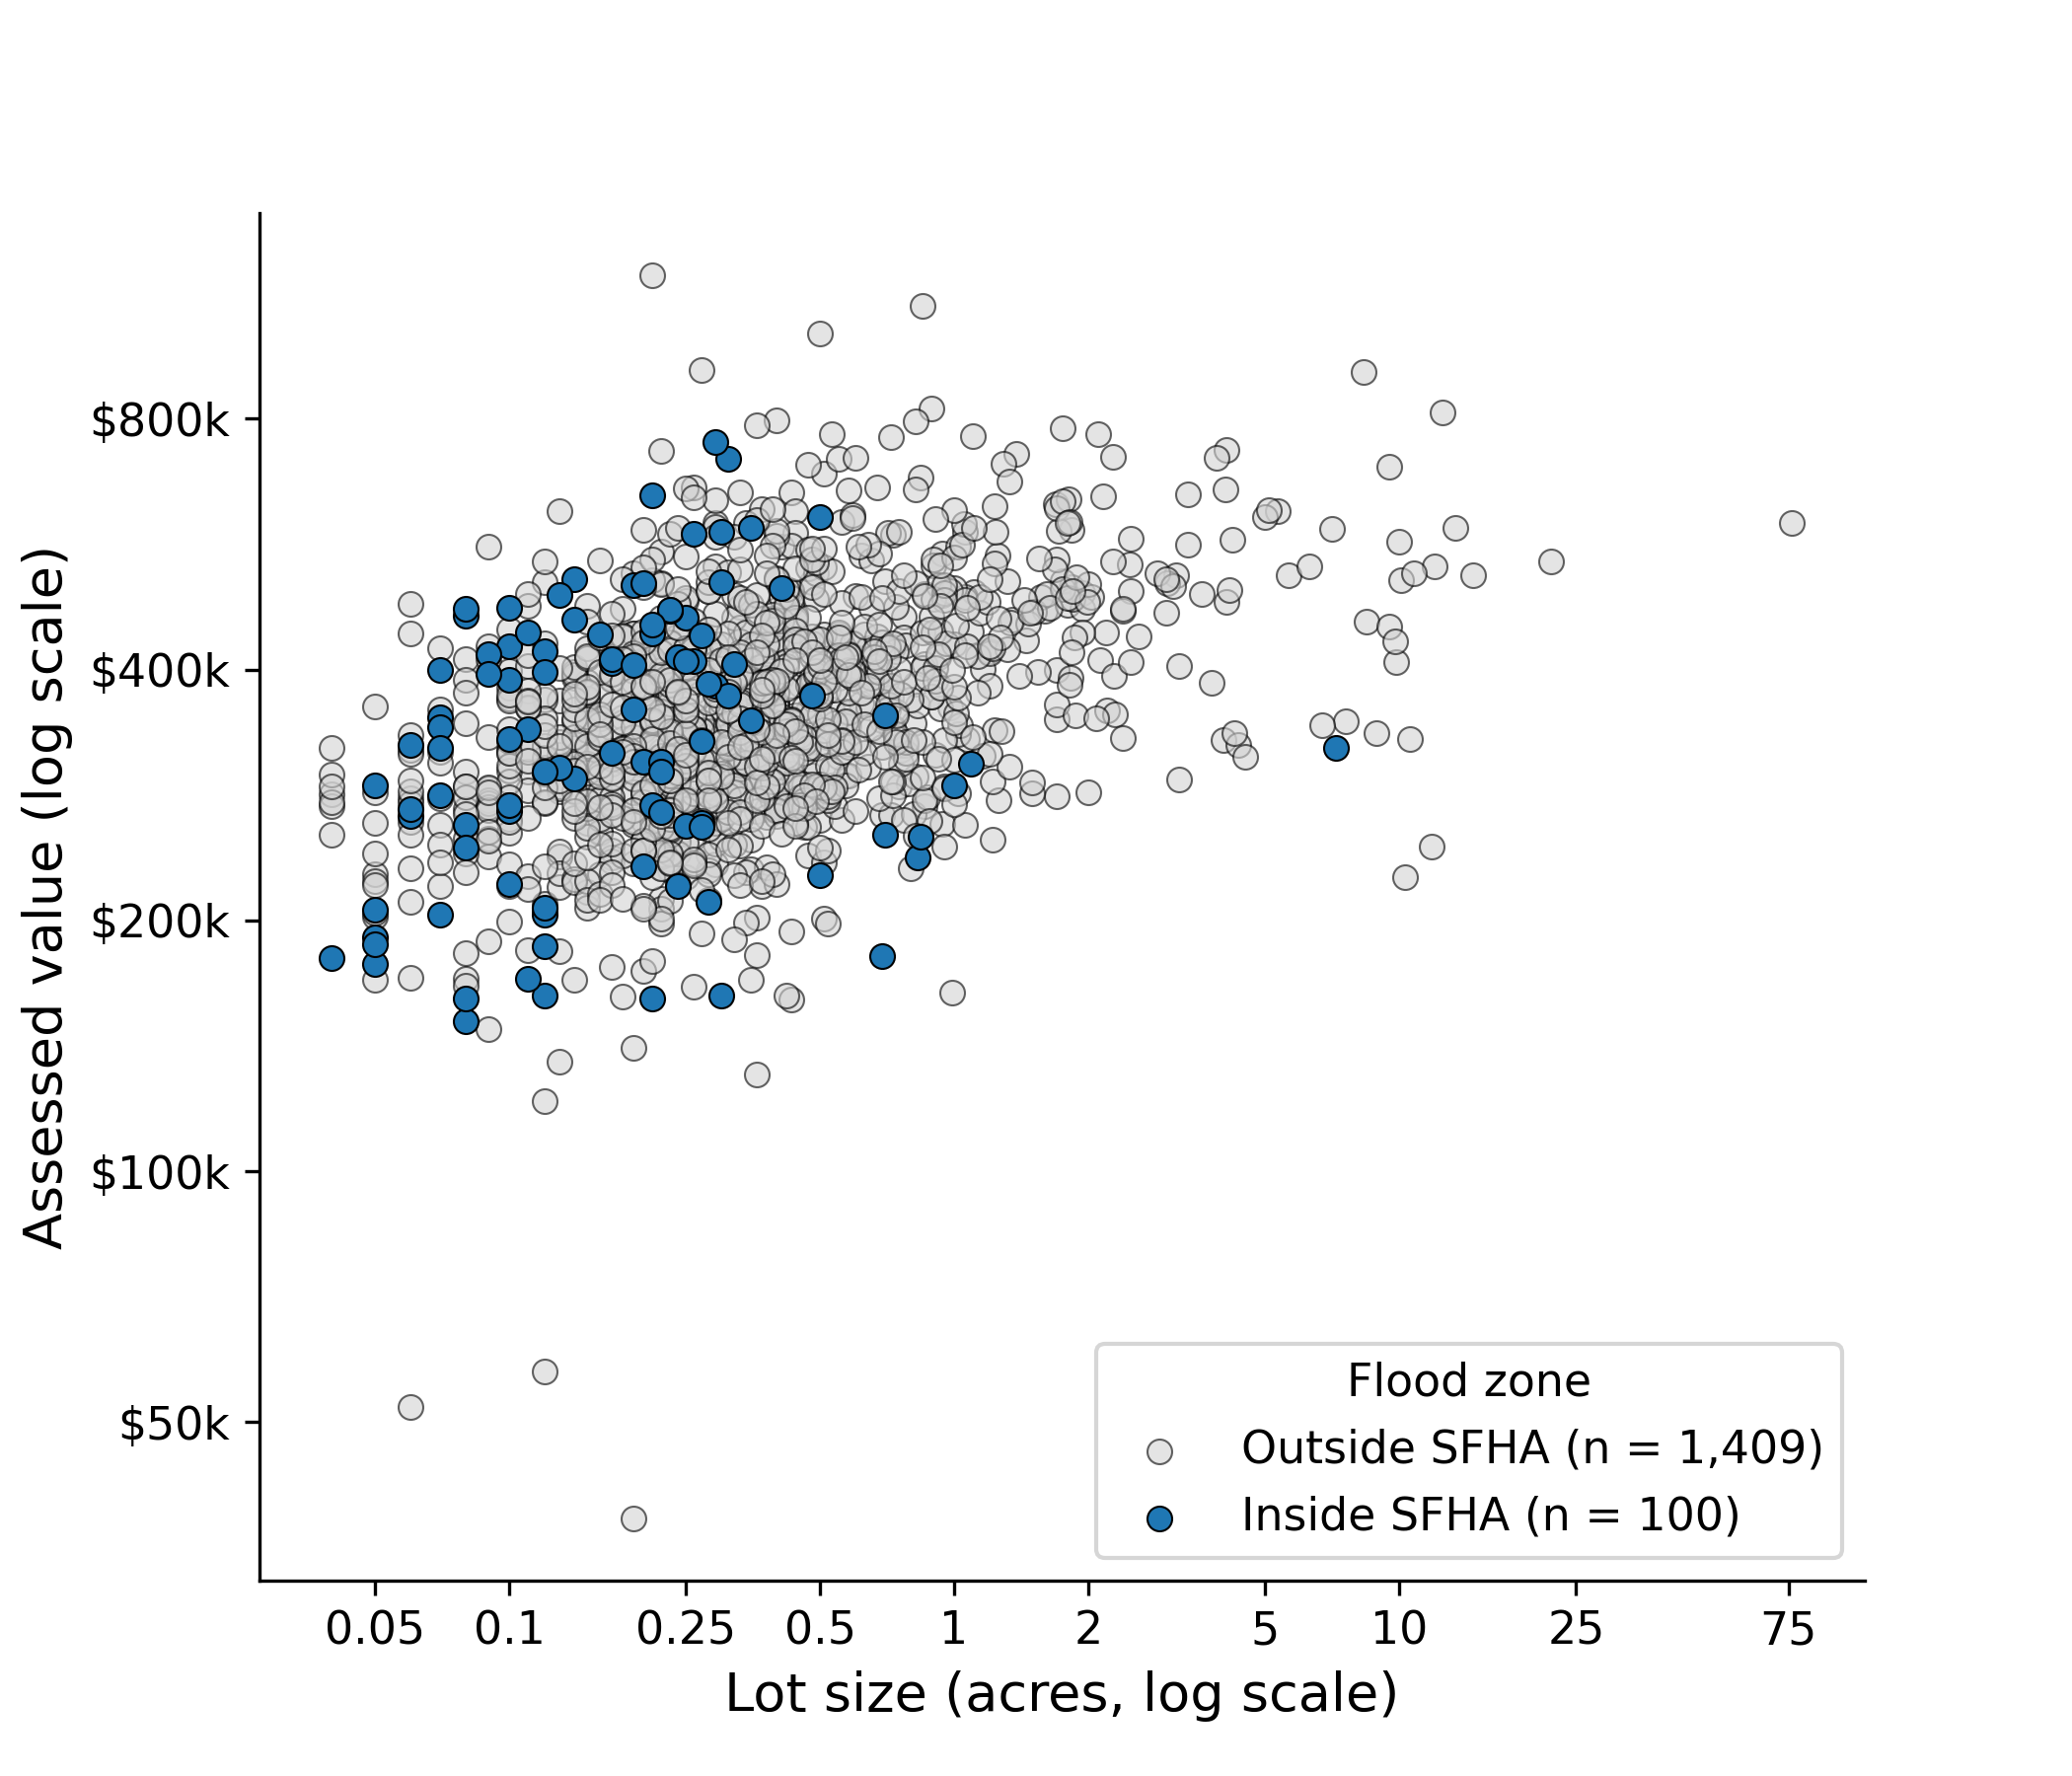
\includegraphics[width=0.65\linewidth]{figures/assessed_value_vs_lot_size_montpelier.png}
\caption{\textbf{Assessed Value vs. Lot Size Montpelier} In this plot, we compare lot size on the x-axis to the assessed value of a home on the y-axis (log scale). A gray dot indicates a home is not in the flood zone and a blue dot indicates a home is inside the flood zone. Though the clustering is tight, regardless of flood zone status, the price of a home does trend upward with the size of the lot.}
\label{fig:assessed_value_vs_lot_size_montpelier}
\end{figure}

\section*{Modeling Question}
Are homes in Montpelier's FEMA flood hazard area assessed differently from homes outside it, on lots of the same size, and by how much?

\section*{Modeling Description}
We model assessed value on the log scale, so coefficients act multiplicatively on dollars. Lot size enters as log acres, centered at its mean, so the intercept describes a home on a typical (geometric-mean, 0.35-acre) lot.

For each parcel $i = 1, \dots, 1509$: $Y_i$ is the log assessed value, $X_{i1}$ is 1 if the home's footprint intersects a FEMA flood hazard area and 0 otherwise, and $X_{i2}$ is centered log lot size.

$$Y_i\sim\mathrm{Normal}(\mu_i,\sigma) \quad \text{(likelihood)}$$
$$\mu_i = \alpha + \beta_1 X_{i1} + \beta_2 X_{i2}$$
$$\alpha\sim \mathrm{Normal}(12, 0.5) \quad \text{(prior)}$$
$$\beta_j \sim\mathrm{Normal}(0,0.5), \ j = 1, 2 \quad \text{(prior)}$$
$$\sigma \sim\mathrm{Exponential}(3) \quad \text{(prior)}$$

$\alpha$: expected log value of a home outside the flood zone on a typical lot.

$\beta_1$: difference in expected log value between homes in and out of the flood zone, on lots of the same size.

$\beta_2$: change in expected log value per unit of log lot size, i.e. how value scales with lot size.

$\sigma$: standard deviation of log values around the regression line, assumed the same for homes in and out of the flood zone.

$\alpha, \beta_1, \beta_2$ can take any real value; $\sigma > 0$. In the Stan output, `beta[1]` is $\beta_1$ and `beta[2]` is $\beta_2$. The prior choices are justified in the \ref{sec:Prior-predictive Analysis} section .

\section*{Prior-predictive Analysis} \label{sec:Prior-predictive Analysis}
\begin{figure}[H]
\centering
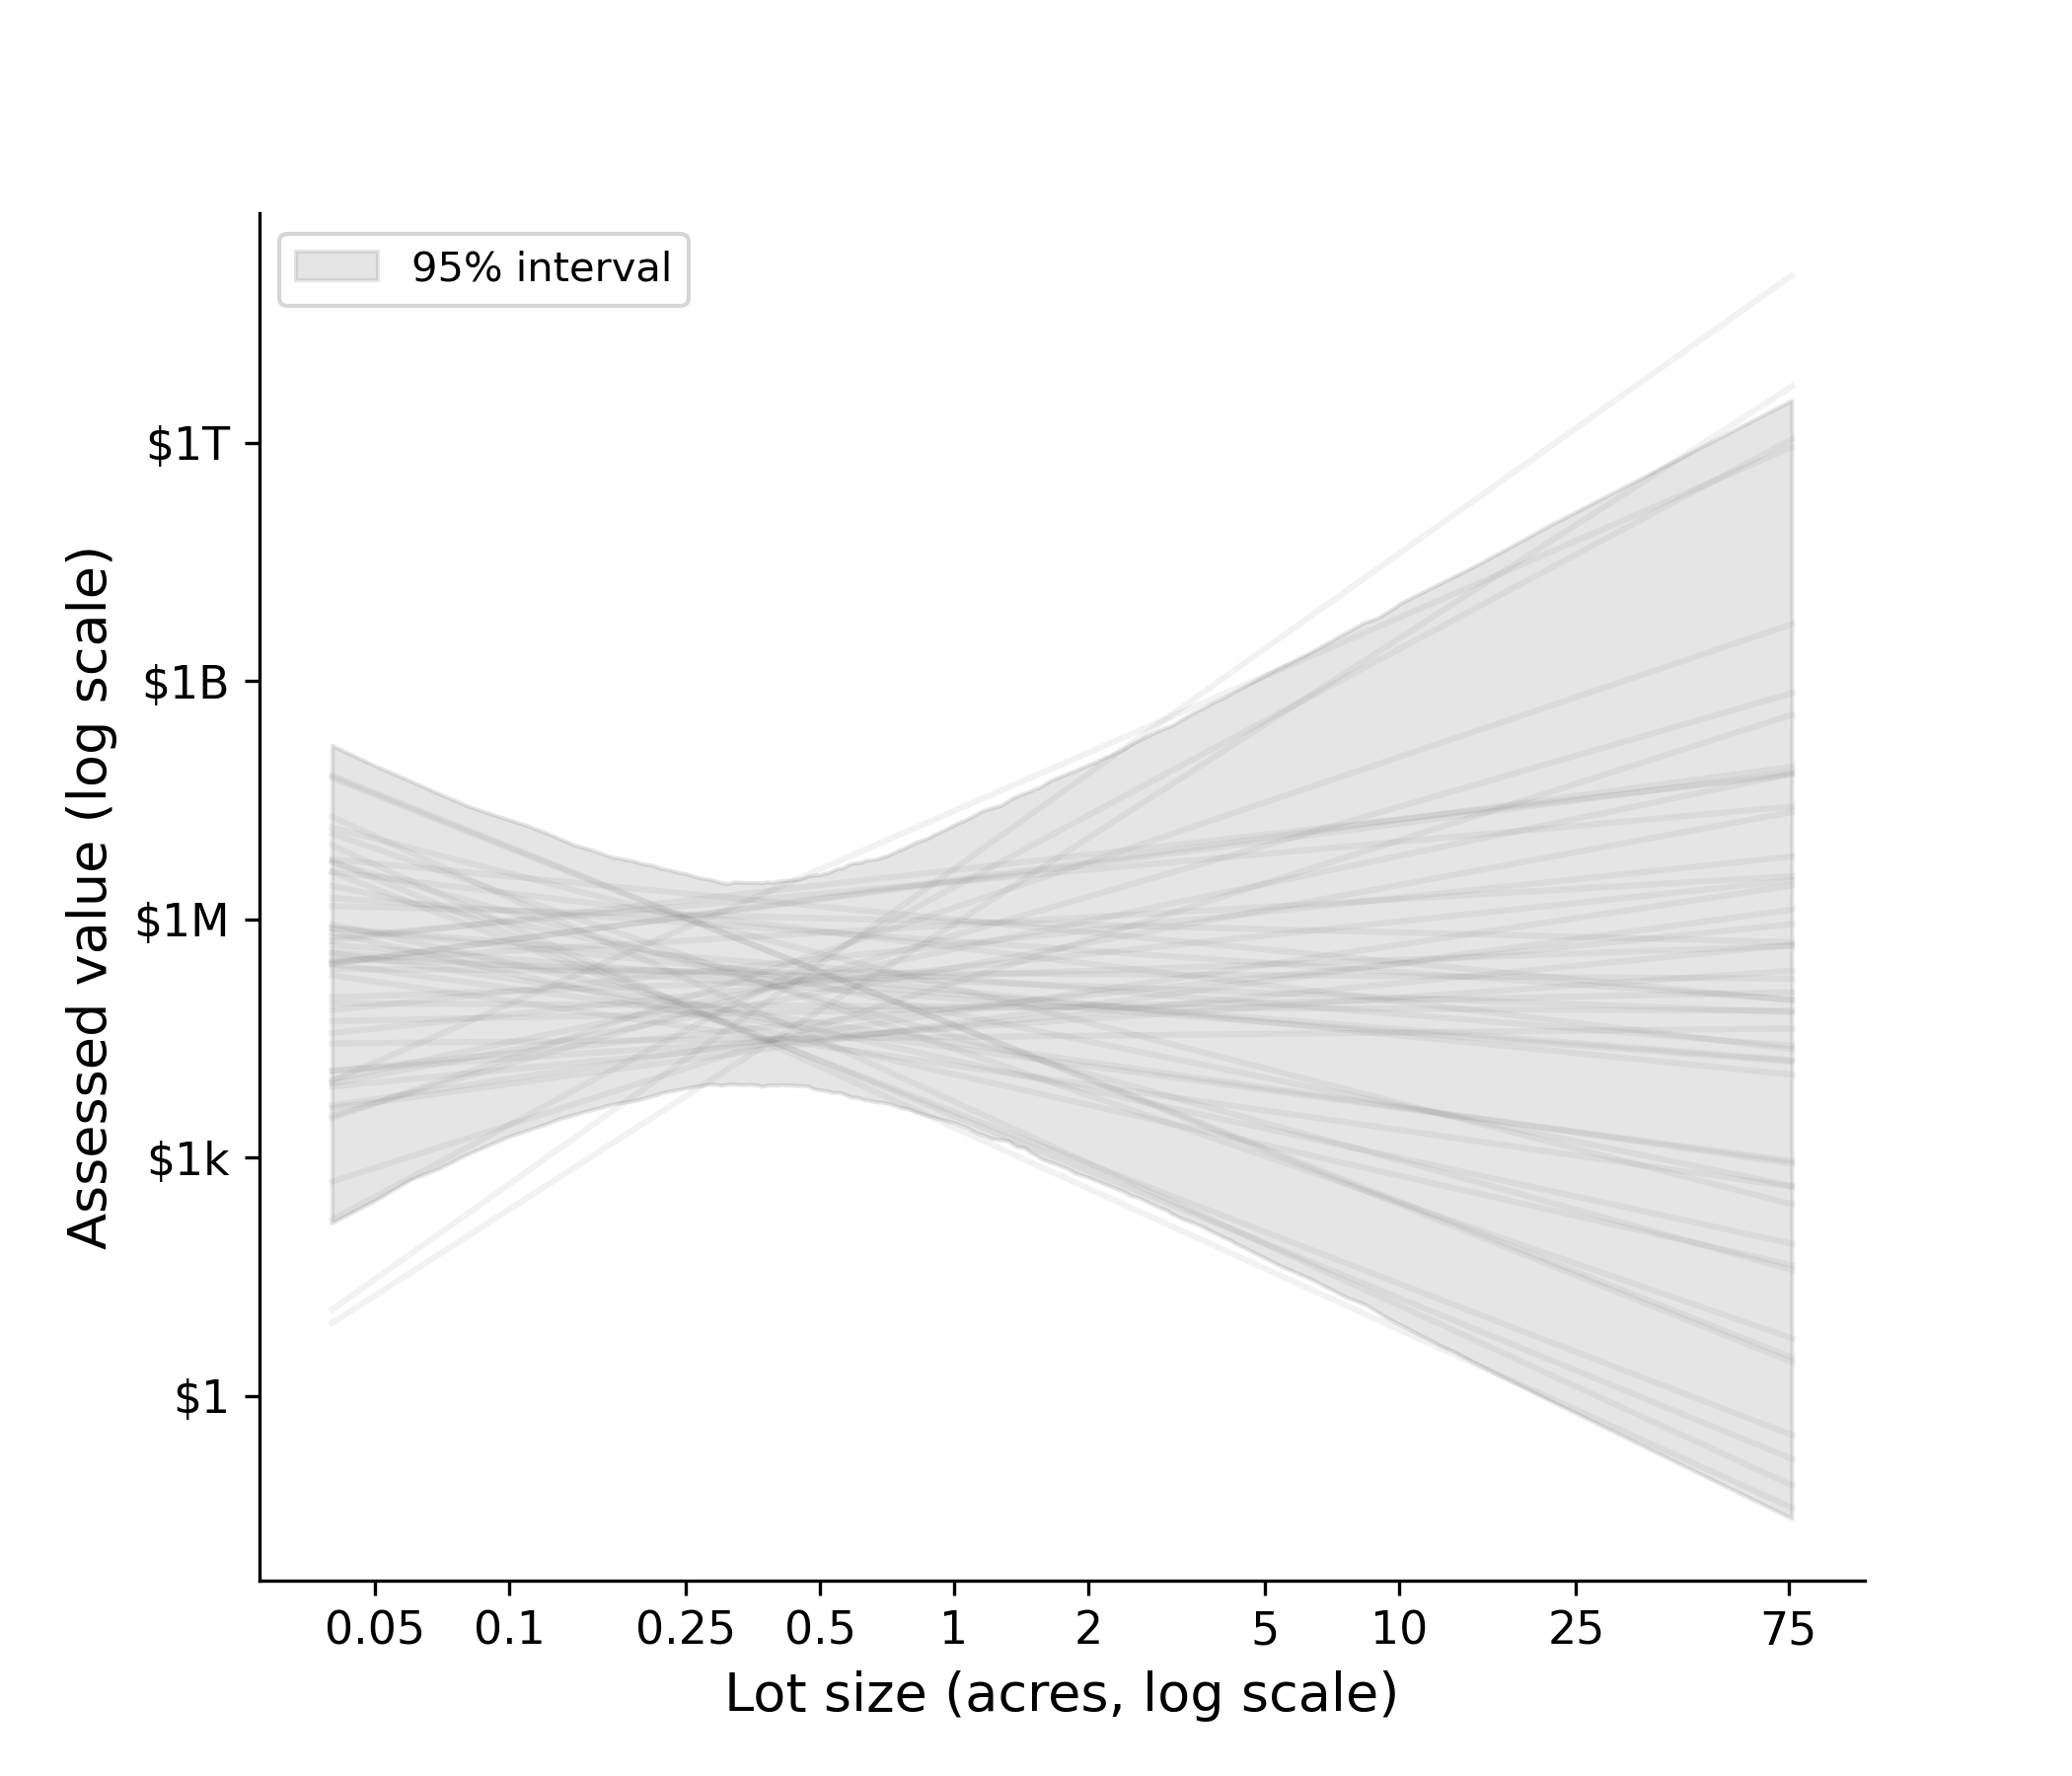
\includegraphics[width=0.75\linewidth]{figures/prior_regression_lines_candidate_1.png}
\caption{\textbf{Prior regression lines, candidate 1:} $\alpha \sim \mathrm{Normal}(12, 1.5)$, $\beta_j \sim \mathrm{Normal}(0, 1.5)$, $\sigma \sim \mathrm{Exponential}(3)$. Grey lines are 50 draws of the mean log value for homes outside the flood zone. The shaded region is the 95\% interval. Lines cluster tightly around the typical 0.35-acre lot, where the band spans roughly \$8k to \$3.3M, and fan out to under \$1 and over \$1T at the largest lots. These extreme values are impossible. }
\label{fig:prior_regression_lines_candidate_1}
\end{figure}

\section*{Prior-predictive Analysis}
\begin{figure}[H]
\centering
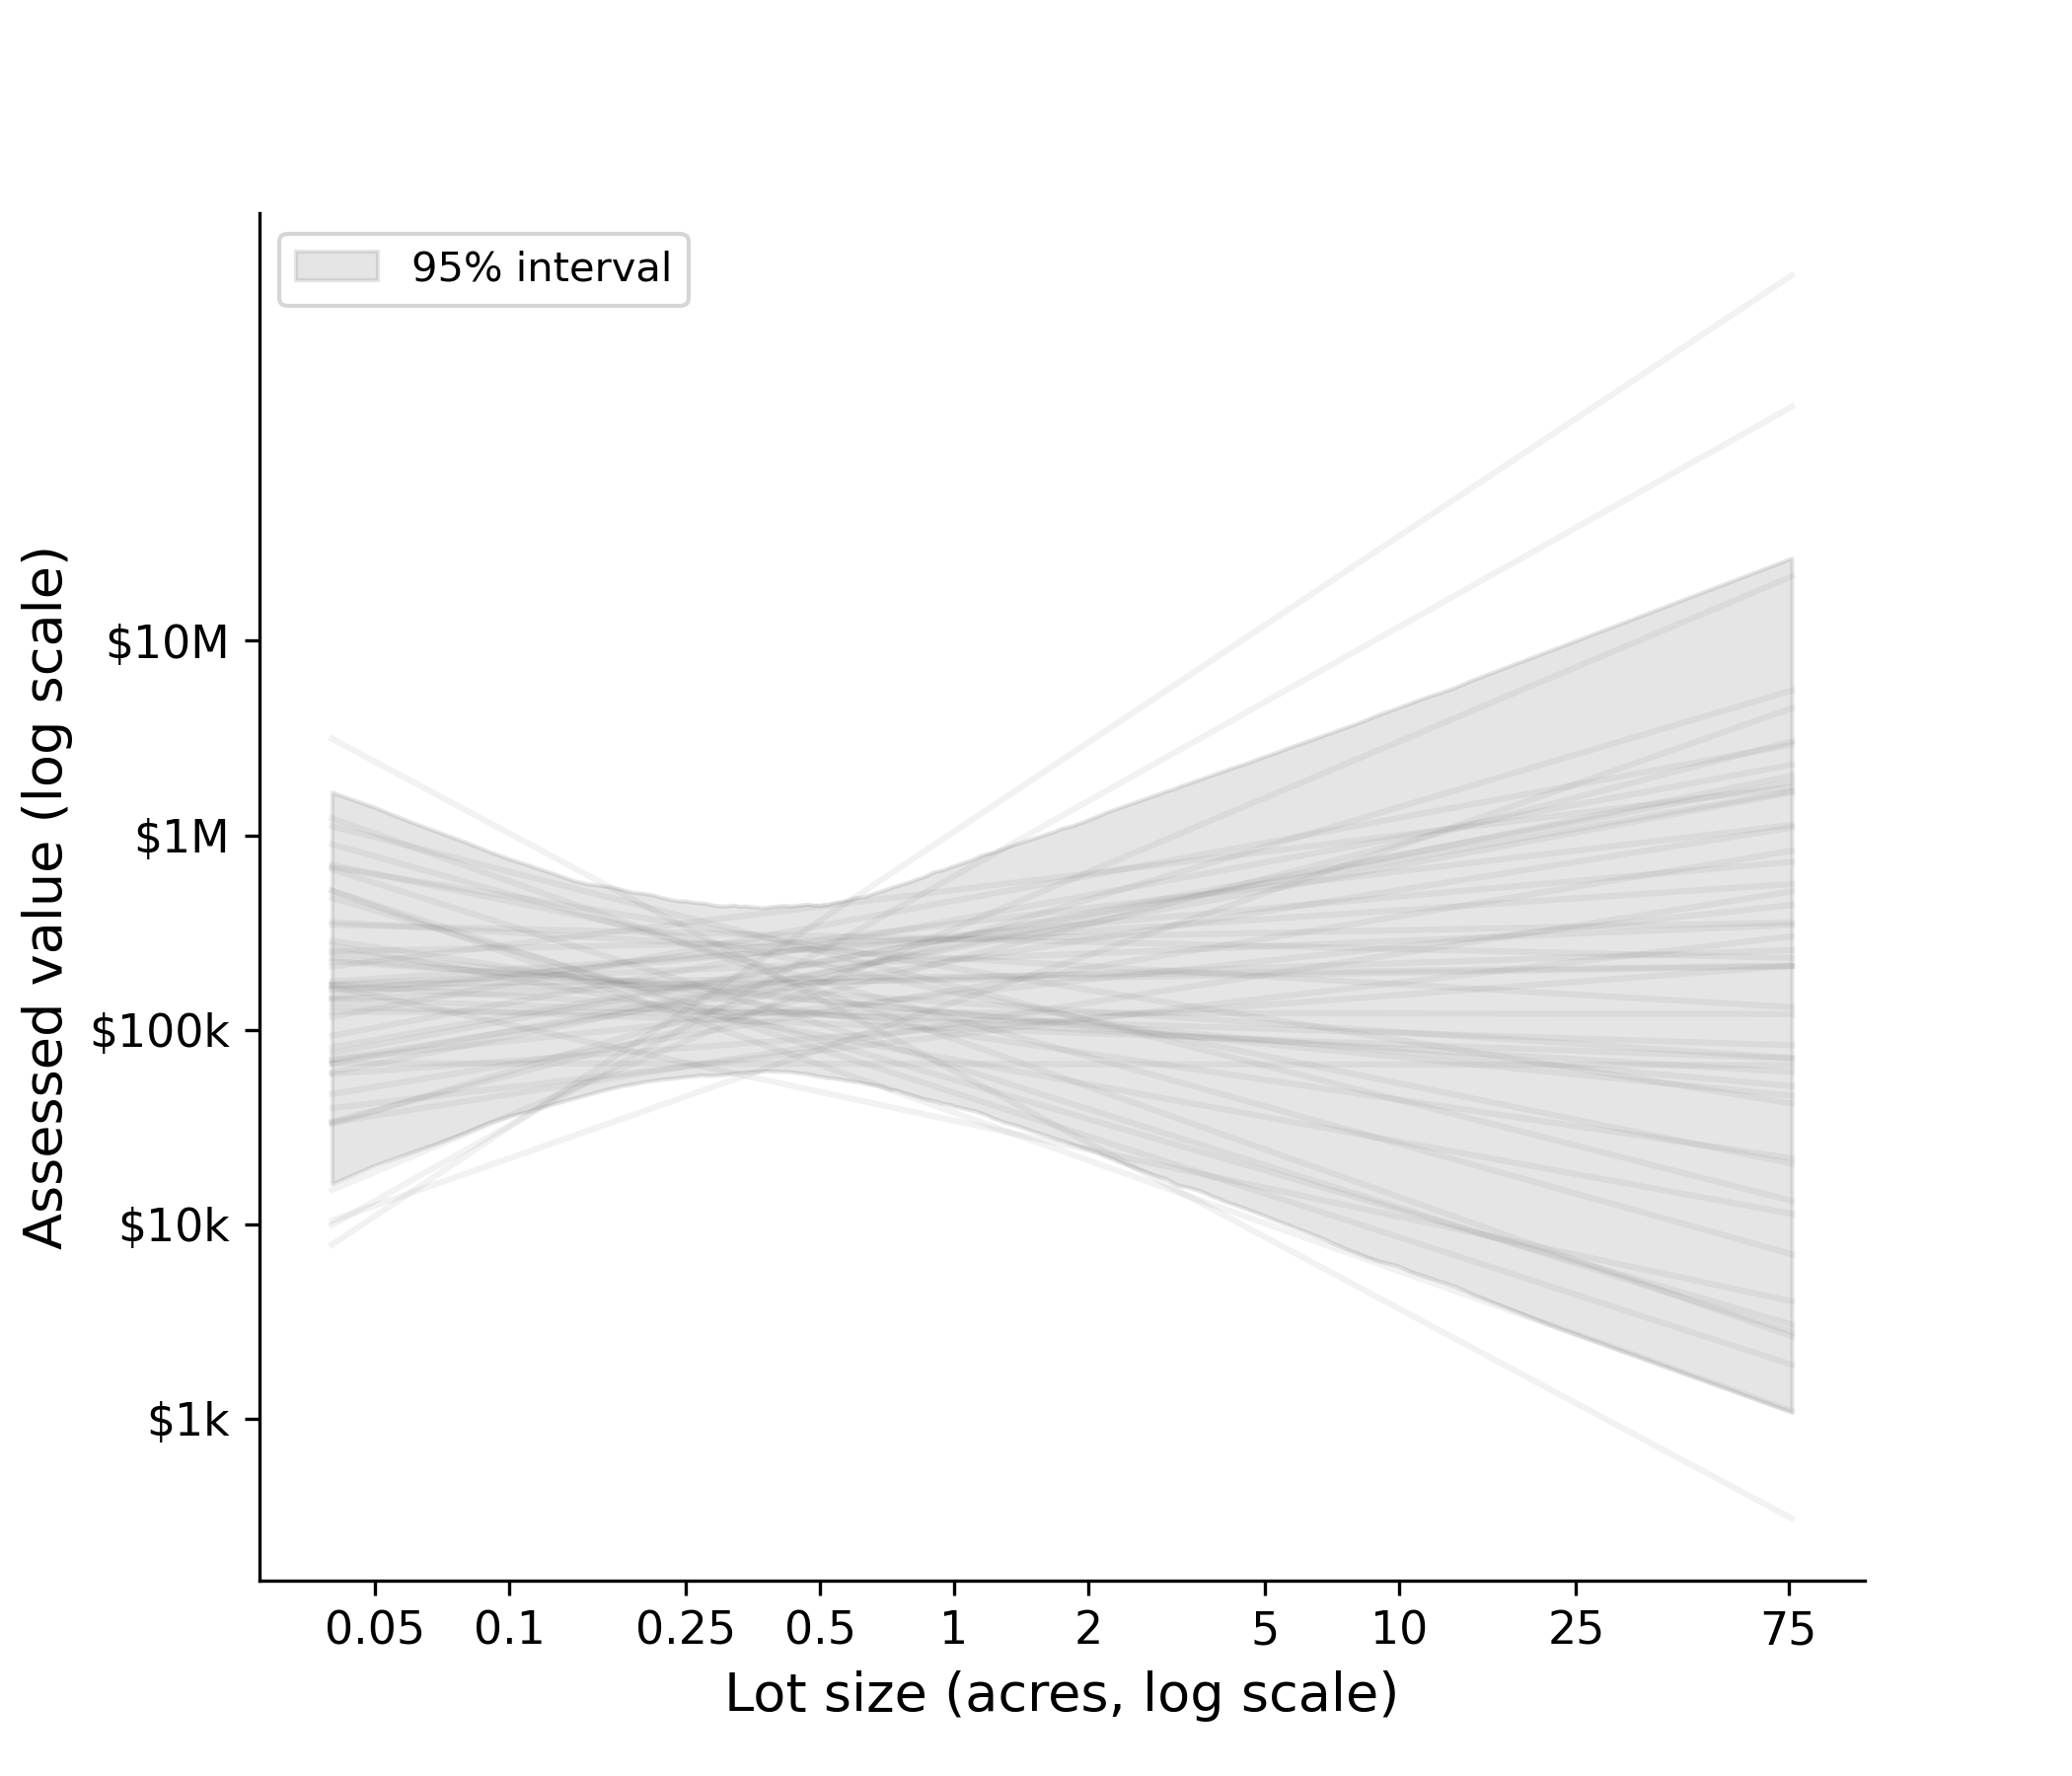
\includegraphics[width=0.75\linewidth]{figures/prior_regression_lines_candidate_2.png}
\caption{\textbf{Prior regression lines, candidate 2:} $\alpha \sim \mathrm{Normal}(12, 0.5)$, $\beta_j \sim \mathrm{Normal}(0, 0.5)$, $\sigma \sim \mathrm{Exponential}(3)$. Grey lines are 50 draws of the mean log value for homes outside the flood zone. The shaded region is the 95\% interval. Lines cluster tightly around the typical 0.35-acre lot, where the band spans roughly \$60k to \$428k.}
\label{fig:prior_regression_lines_candidate_2}
\end{figure}

\begin{figure}[H]
\centering
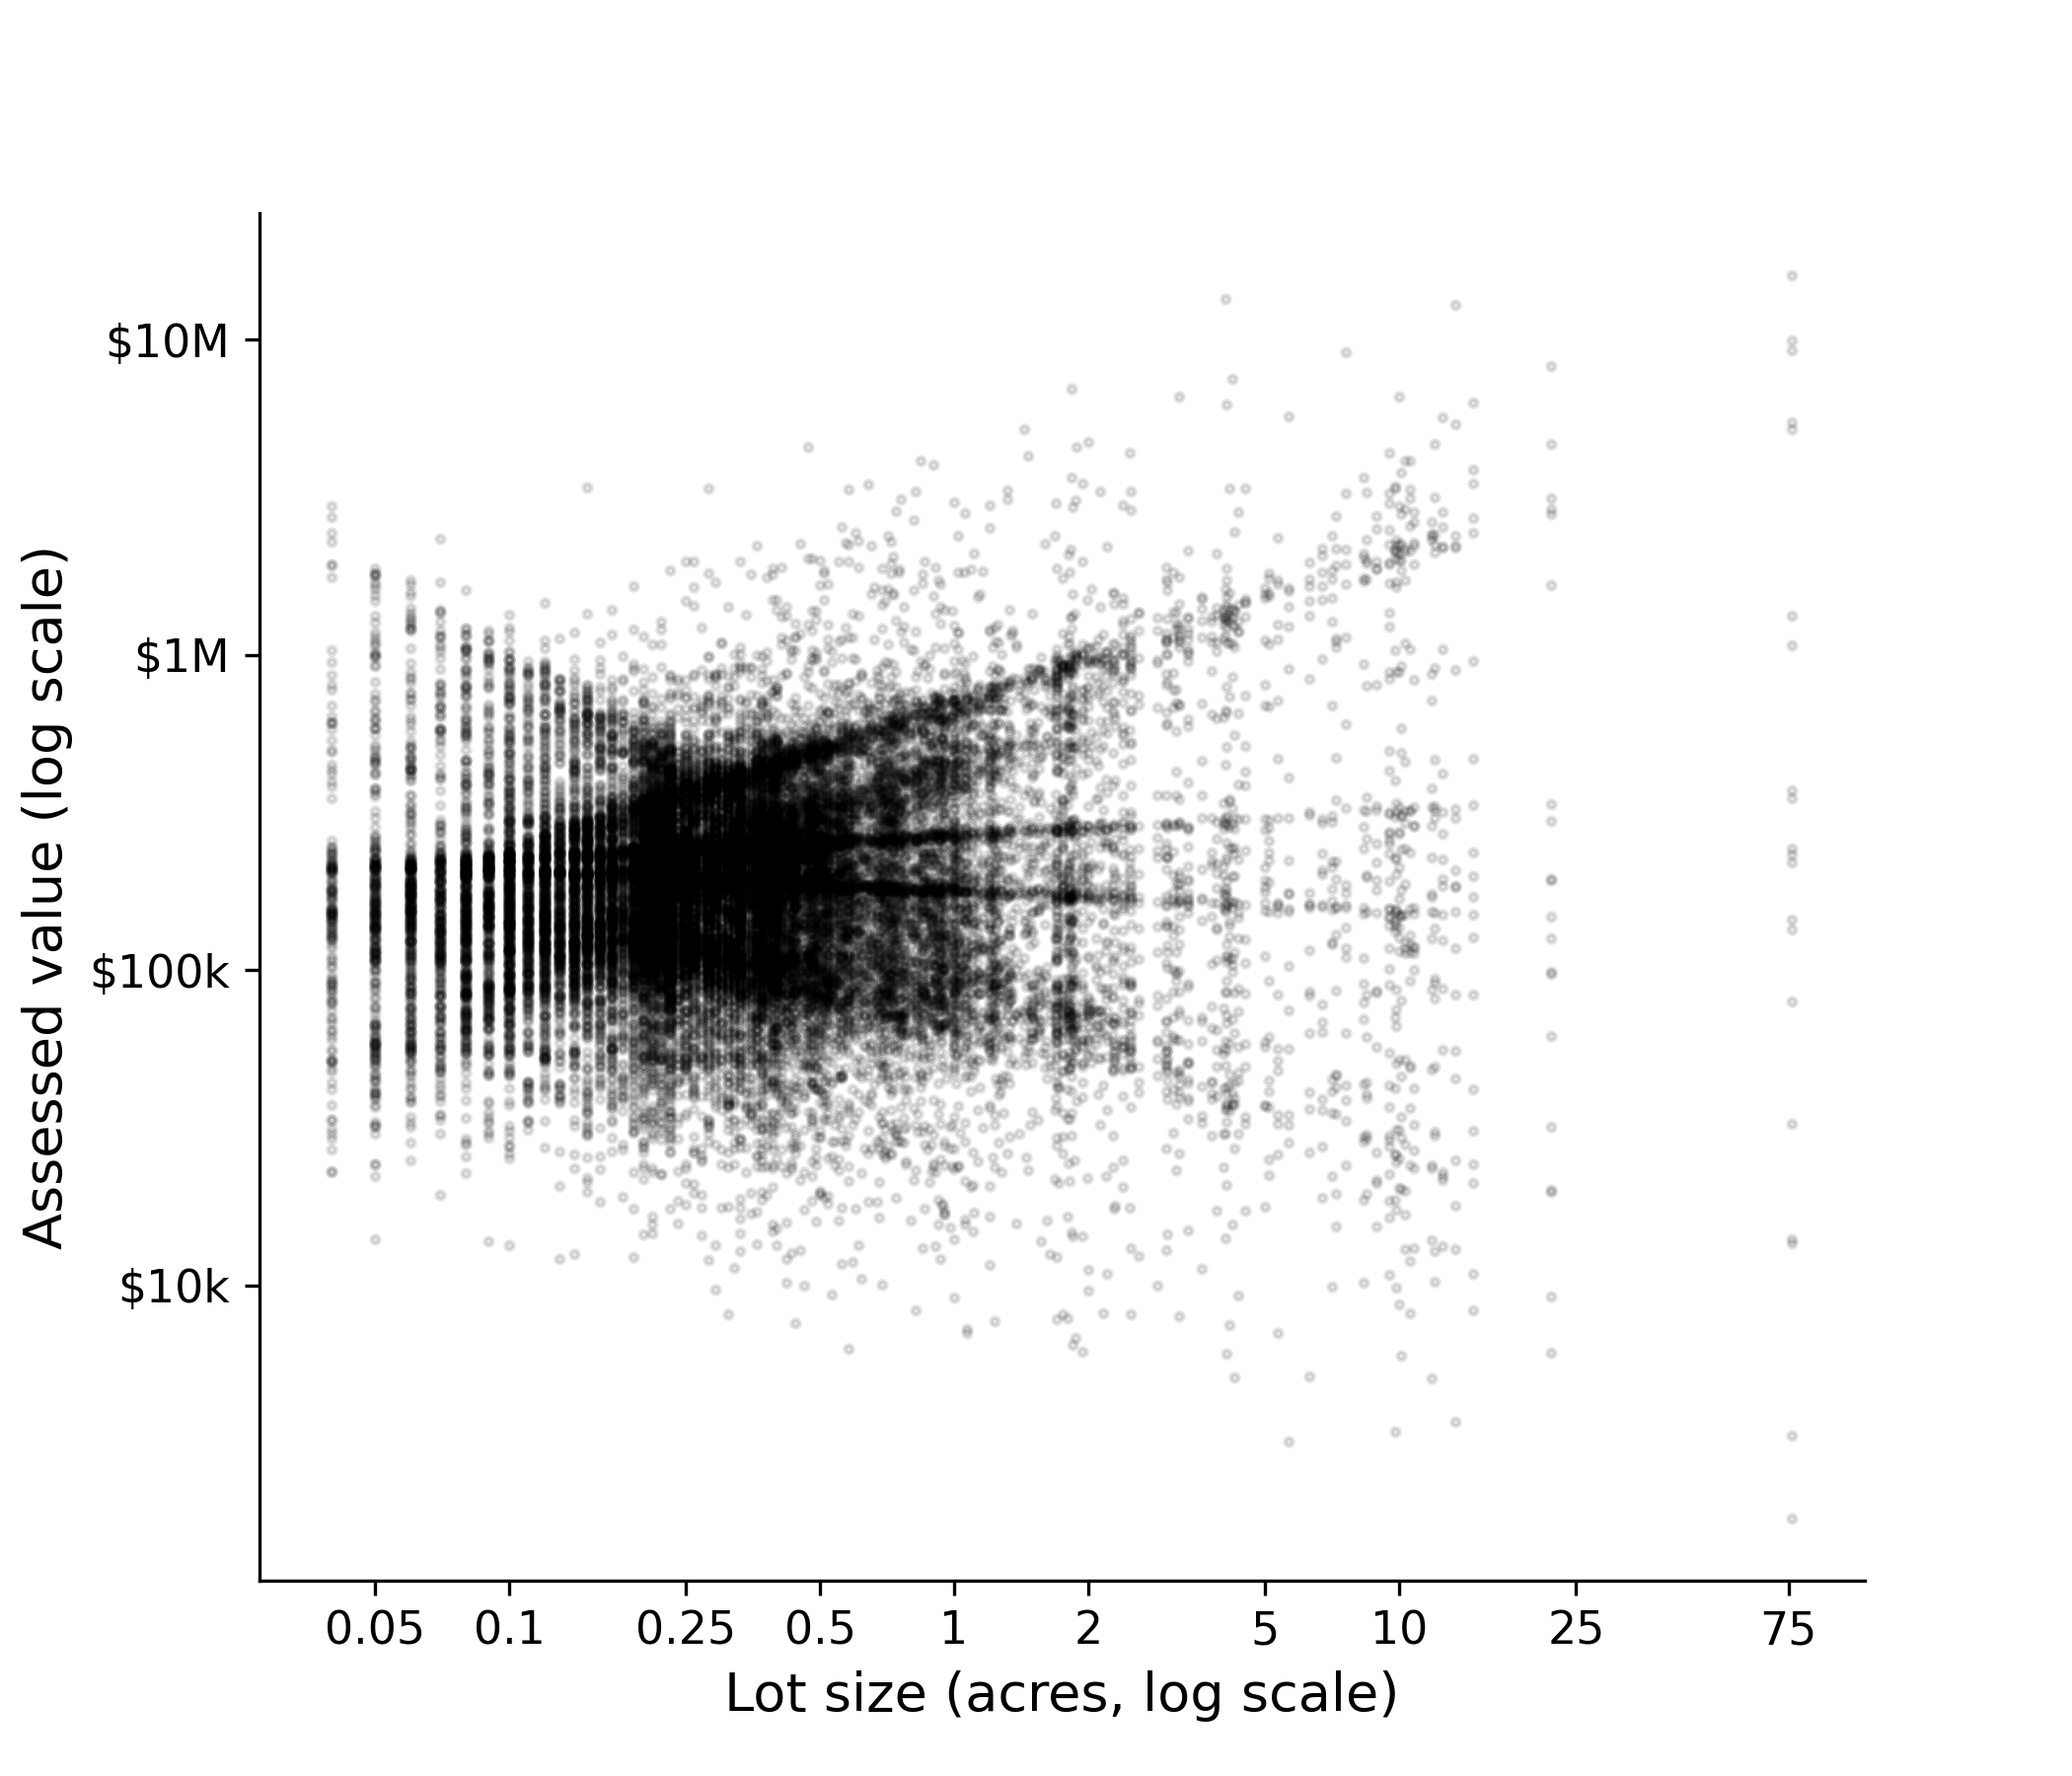
\includegraphics[width=0.75\linewidth]{figures/prior_predictive_datasets_candidate_2.png}
\caption{\textbf{Prior predictive datasets, candidate 2} 20 datasets are simulated from the prior. Each uses the observed lot size. Most simulated homes fall within a reasonable range between \$10k and $160k.$. The prior produces a few extreme values on larger lots.}
\label{fig:prior_predictive_datasets_candidate_2}
\end{figure}

\section*{Estimation}

\begin{table}[H]
\centering
\begin{tabular}{lcc}
\hline
Parameter & Posterior mean & 95\% credible interval \\
\hline
$\alpha$ & 12.766 & [12.752, 12.780] \\
$\beta_1$ (flood) & 0.028 & [$-0.031$, 0.088] \\
$\beta_2$ (lot size) & 0.141 & [0.126, 0.156] \\
$\sigma$ & 0.285 & [0.275, 0.295] \\
\hline
\end{tabular}
\caption{Posterior means and central 95\% credible intervals (log scale). All $\hat{R} \le 1.003$; bulk ESS $\approx 2{,}000$; no divergences or other sampler warnings.}
\end{table}



\begin{figure}[H]
\centering
\includegraphics[width=.99\linewidth]{figures/pairplot_multiple_fit.png}
\caption{\textbf{Posterior Distribution of $\alpha$, $\beta$, and $\sigma$}}
\label{fig:pairplot_multiple_fit}
\end{figure}

\section*{Posterior Predictive Check}

\begin{figure}[H]
\centering
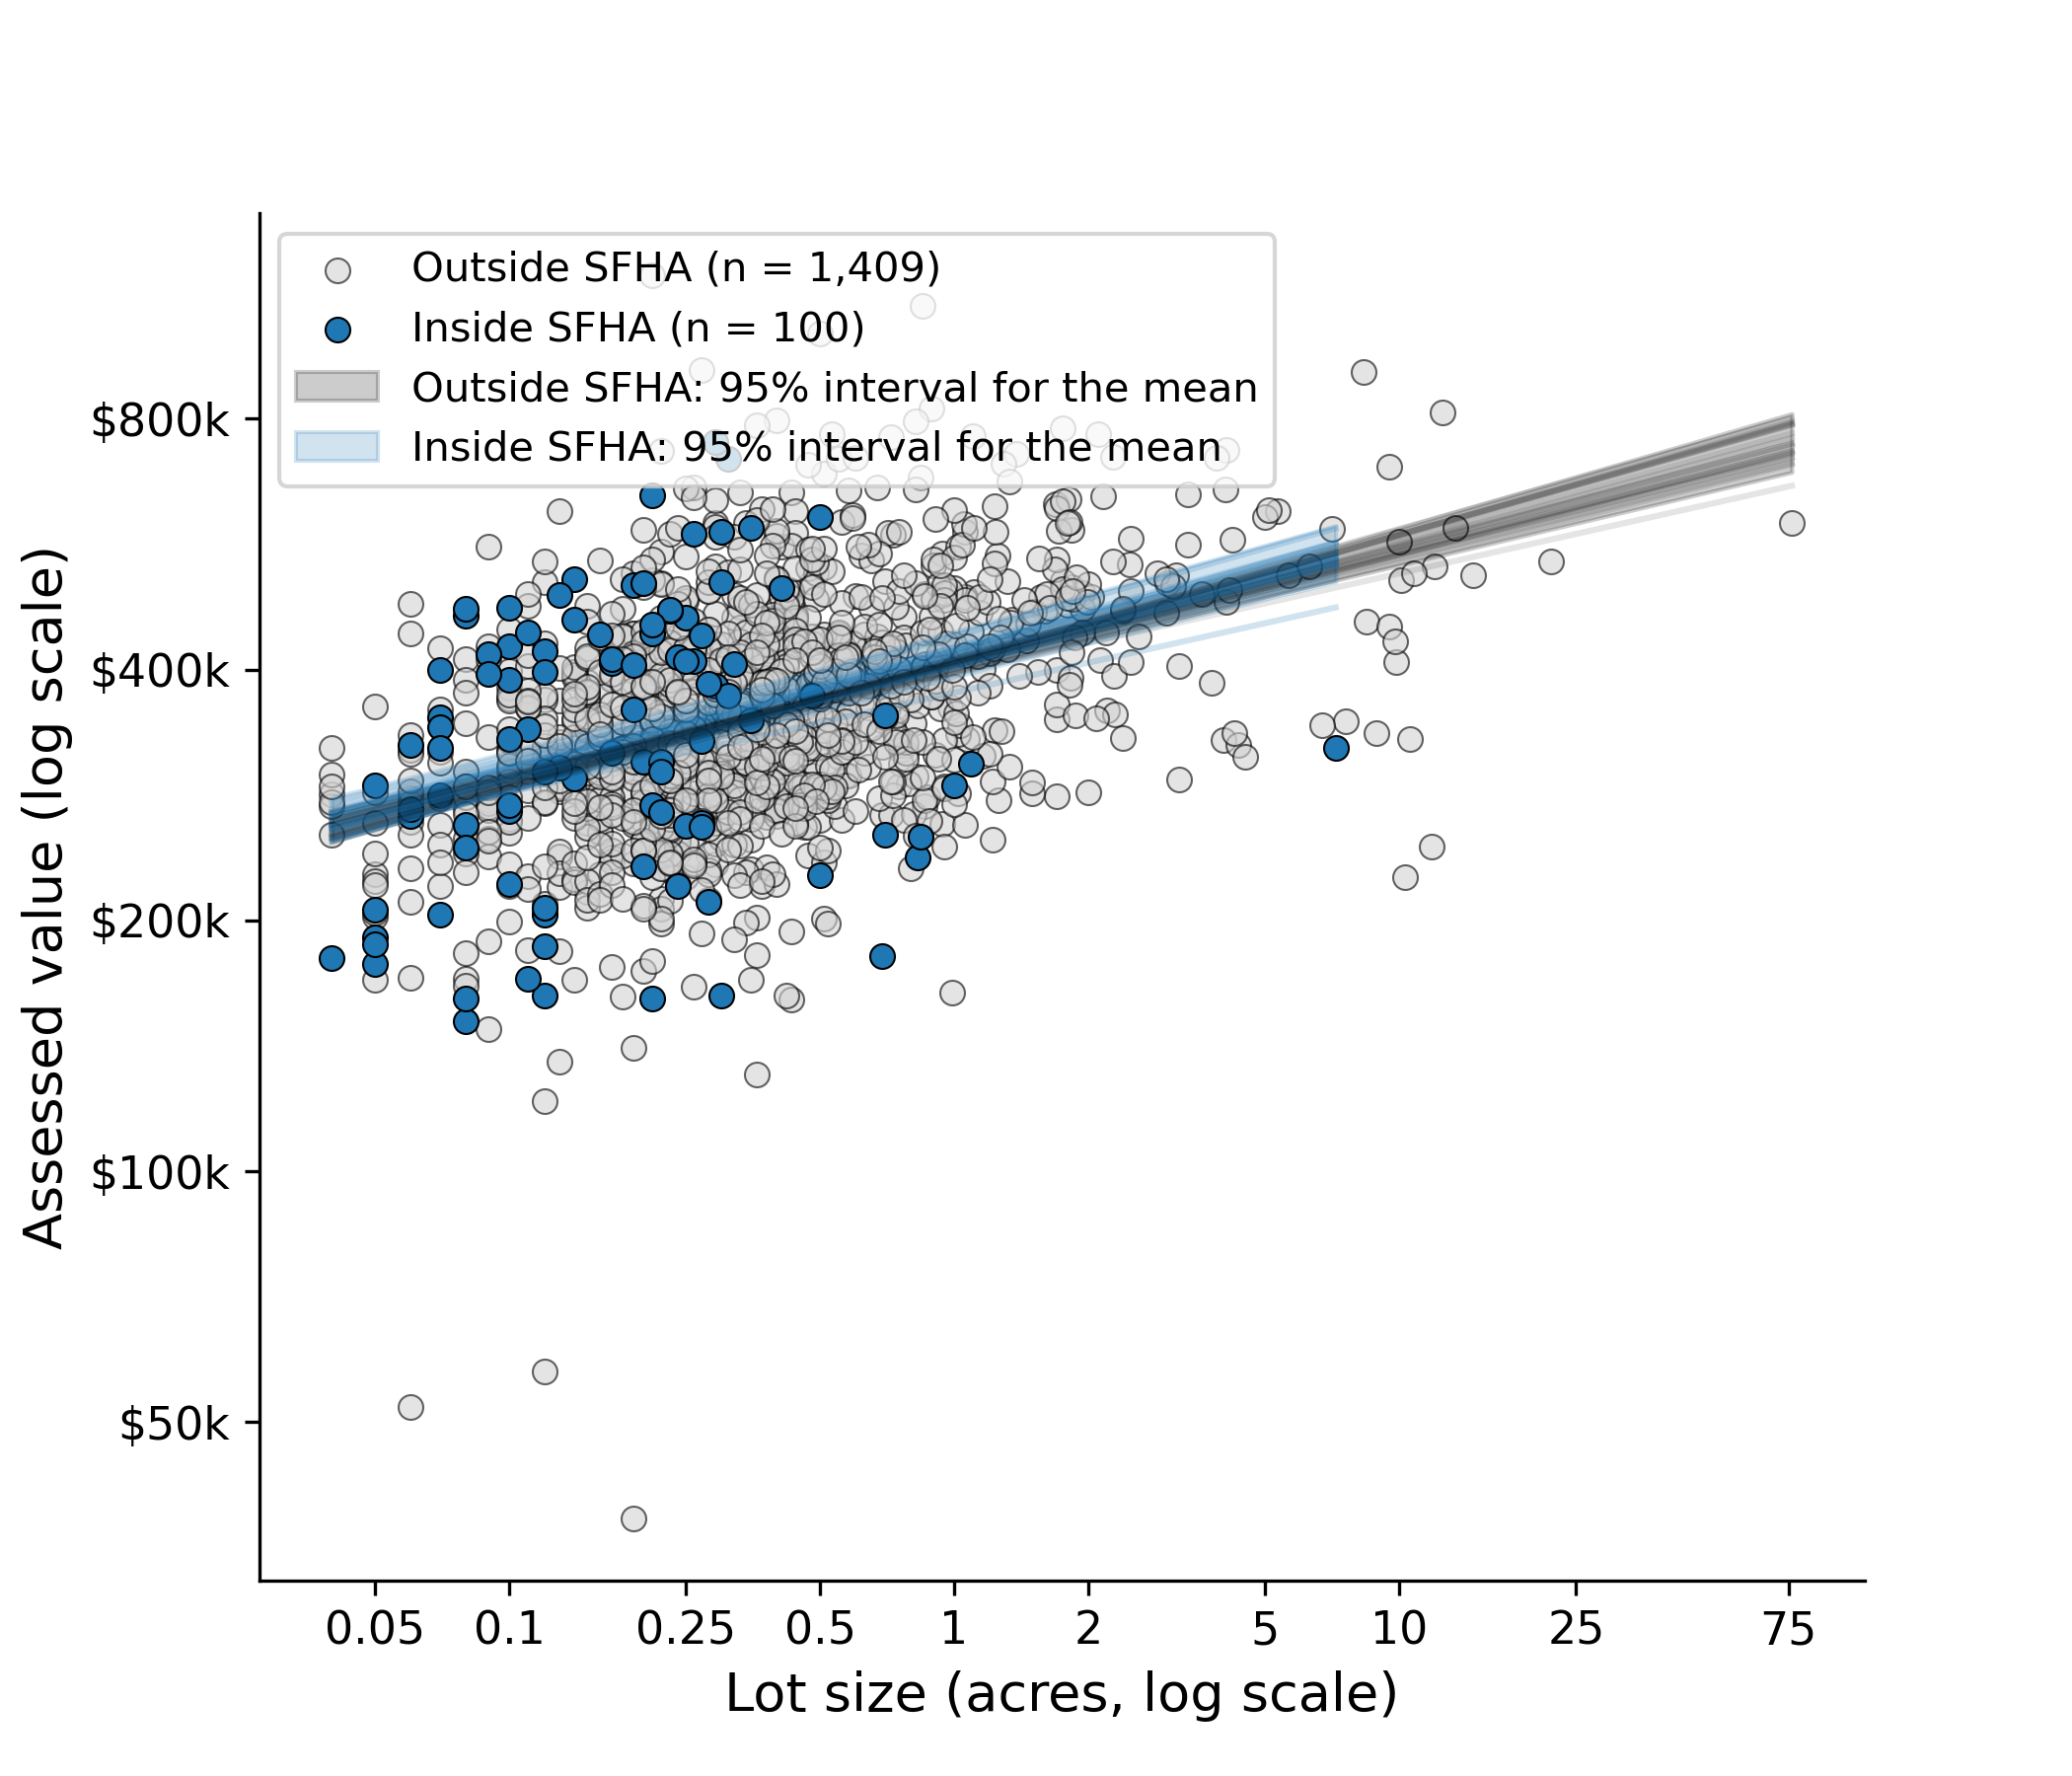
\includegraphics[width=.75\linewidth]{figures/posterior_regression_lines.png}
\caption{}
\label{fig:posterior_regression_lines}
\end{figure}

\begin{figure}[H]
\centering
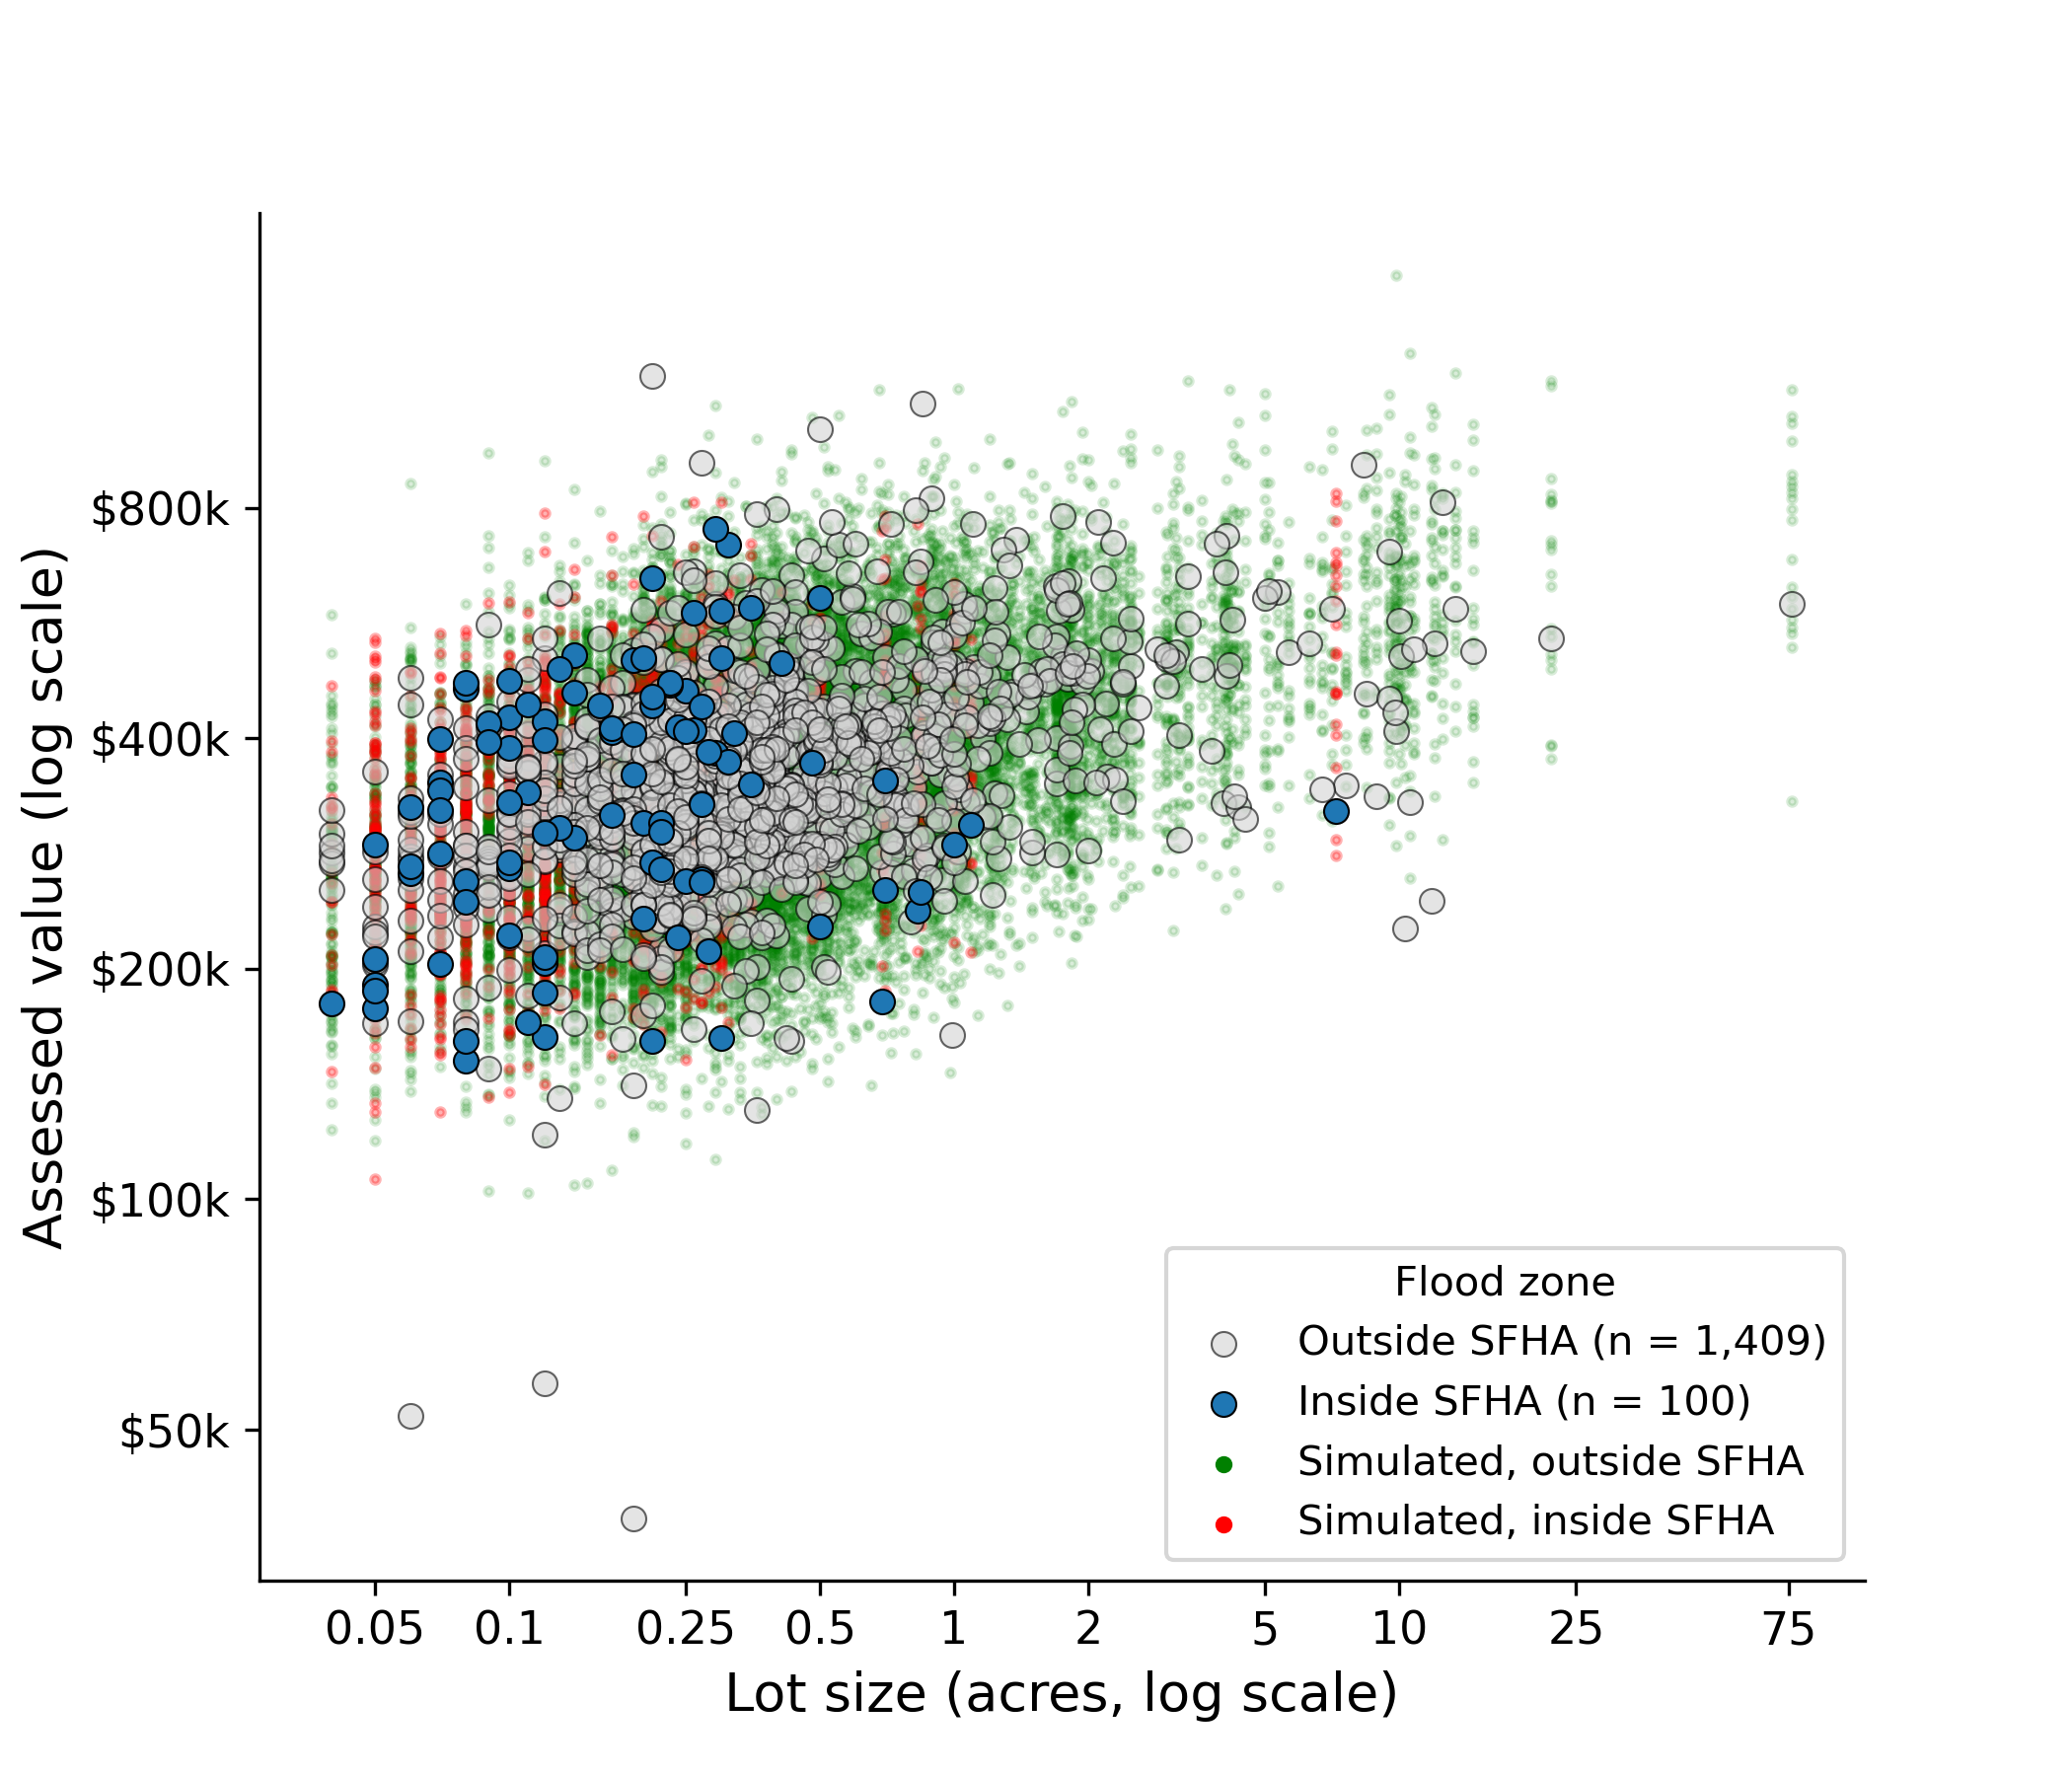
\includegraphics[width=.75\linewidth]{figures/posterior_predictive_datasets.png}
\caption{}
\label{fig:posterior_predictive_datasets}
\end{figure}

\section*{Interpretation}
\section*{Self-assessment}
\section*{Declaration of AI Use}

\bibliographystyle{plainnat}
\bibliography{project}

\end{document}
